% !TEX root = template.tex

\section{Processing Pipeline}
\label{sec:processing_architecture}

Analysis of raw data coming from IMU sensors generally follows a \mbox{pipeline-based} approach composed of different blocks. \fig{fig:img_pipeline} shows a schematic representation of the preprocessing and classification phases.

\begin{figure}[h]
	\captionsetup{font=scriptsize, justification=centering}
    \centering
	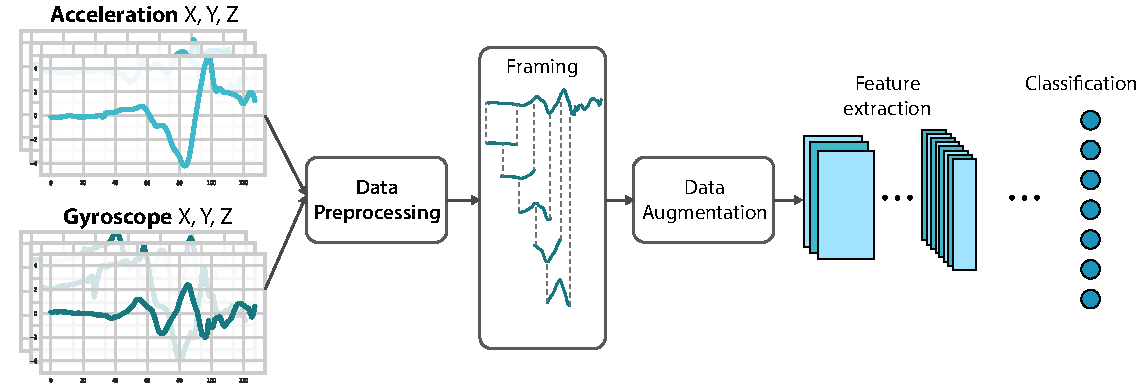
\includegraphics[width=\columnwidth]{pipeline}
    \caption{Schematic representation of the processing pipeline.}
    \label{fig:img_pipeline}
\end{figure}

Time series data from the IMU sensors is converted into contiguous segments through a \mbox{sliding-window} approach, the output of this process are feature vectors which represent the input of the machine learning models. Once the dataset is created, it is augmented and divided in training and test set and finally normalized with respect to the mean and variance of the training set. The basic blocks of all the approaches mentioned in this paper are the ones which typically constitute a CNN. Each CNN contains at least one convolution layer along the temporal domain, one pooling layer and at least one fully connected layer prior to a softmax layer. In the convolutional layer, a mathematical operation (i.e. convolution) applies a set of local filters (or kernels) to obtain the most representative features. After the convolution operation, a bias is added to the result. Subsequent \mbox{max-pooling} operations look for the maximum within a region of specific width and height, this corresponds to a subsampling which introduces translational invariance to the system and improves its robustness. The fully connected layer is applied at the end, combining all features' maps obtained by the previous convolutional steps and using it as input for a 7 neurons softmax layer which computes the probability of each activity class. Regularization techniques such as dropout, early stopping and batch normalization are used at different stages of the neural network in order to avoid overfitting to the training data. \par
Stacked denoising convolutional autoencoders (SDAs) are built on the same basic blocks mentioned above but follow a slightly different processing pipeline. \fig{fig:img_ae} represents the structure of a stacked autoencoder. The main building block is the autoencoder which can be separated into two parts, an encoder and a decoder. The encoder part consists of convolution layers and \mbox{fully-connected} layers and the decoder part consists of \mbox{fully-connected} layers and deconvolution layers. An ordinary autoencoder where the output $Y$ is of the same dimensionality as input $X$ can achieve perfect reconstruction simply by learning an identity mapping. This criterion alone is unlikely to lead to the discovery of a more useful representation ofthe input. The traditional approach to autoencoders uses a bottleneck to produce an \mbox{under-complete} representation, the resulting $Y$ can thus be seen as a lossy compressed representation of $X$. Since the reconstruction criterion alone is unable to guarantee the extraction of useful features, a more challenging and more interesting objective would be to clean a partially corrupted input (denoising). It's important to emphasize that the goal is not the task of denoising per se, rather denoising is investigated as a training criterion for learning to extract useful features that will constitute better higher level representation of the input \cite{Pascal-2010}. A key function of SDAs is unsupervised \mbox{pre-training}. Once each layer is \mbox{pre-trained} to conduct feature selection and extraction on the input from the preceding layer, a second stage of supervised \mbox{fine-tuning} can follow. The unsupervised \mbox{pre-training} of such architecture is done one layer at a time. Each layer is trained as a denoising autoencoder by minimizing the error in reconstructing its input. Once all layers are \mbox{pre-trained}, the network goes through a second stage of training known as supervised \mbox{fine-tuning} whose goal it to minimize prediction error on a supervised task. During this latter supervised phase only the dense layers are trained, while the rest is kept frozen.






\section{Signals and Features}
\label{sec:signals_features}

The dataset used in this paper is taken from \cite{base-paper} \footnote{The dataset is available at http://www.kn-s.dlr.de/activity/}. The IMU used provides the measurements in the sensor frame (SF) and the necessary attitude information in order to rotate them to the global frame. However, acceleration and angular velocity relative to the human body seem to be the most relevant information (and not relative to an earth-fixed reference frame or the sensor frame as the sensor can be placed on the body in any orientation and position) \cite{base-paper}.
The three axes of the body frame are defined to intersect at the sensor location, the z axis is directed towards the head, while the other axis (x and y) form the plane orthogonal to this vertical axis. The sensor was placed on the belt of the test candidates either on the right or the left part of the body.
As shown in \tab{activity_times_table} the final dataset contains over 5 hours of activity data. Class unbalance represents a major obstacle in the classification task. \\

\begin{table}[!htbp]
\captionsetup{font=scriptsize, justification=centering}
\centering
\resizebox{\columnwidth}{!}{%
\begin{tabular}{c|c|c|c|c|c|c|c|}
\cline{2-8}
\textbf{} & \textbf{Standing} & \textbf{Walking} & \textbf{Sitting} & \textbf{Lying} & \textbf{Running} & \textbf{Jumping} & \textbf{Falling} \\ \hline
\multicolumn{1}{|c|}{\textbf{Minutes}} & 121 & 72 & 59 & 28 & 15 & 8 & 2 \\ \hline
\end{tabular}%
}
\caption{Total activity data times for each recorded activity.}
\label{activity_times_table}
\end{table}

The original dataset contains the recordings of one IMU sensor:
\begin{itemize}
\item acceleration values along x-y-z axis
\item gyroscope values along x-y-z axis
\item attitude matrix to convert previous values from sensor to global frame
\item magnetometer values along x-y-z axis
\end{itemize}
Each entry is either labeled with one of the activities among {\it running, jumping, walking, falling, sitting, standing, lying} or as a transition state between these base labels.

\subsection{Data preprocessing}
\label{sec:data_preprocessing}
The current classification task goal is to predict one of the base labels. Detecting transients was out of the scope of this paper and thus they were initially removed from the dataset. One mislabeling error was found and corrected, which was influencing just 5 frames in the original dataset.

\subsection{Framing}
\label{sec:framing}
After the initial preprocessing, next step is to segment the time series data into contiguous segments through a \mbox{sliding-window} approach (\fig{fig:img_framing}).\\

\begin{figure}[h]
	\captionsetup{font=scriptsize, justification=centering}
    \centering
	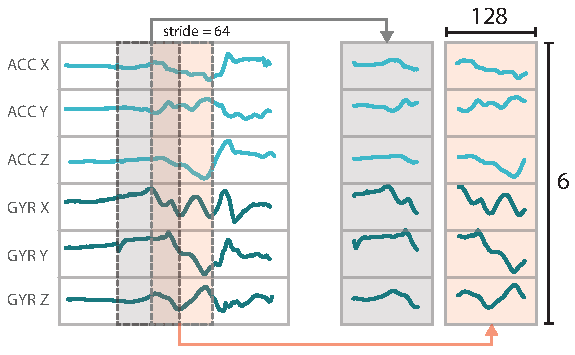
\includegraphics[width=\columnwidth]{framing}
    \caption{Framing procedure.}
    \label{fig:img_framing}
\end{figure}

Each frame or window will be then fed to the machine learning algorithm. Since 1sec is the minimal duration of an activity \cite{base-paper}, I used this as a reference for the window length. The sensor used has a capture rate of 100Hz, which means 100 \mbox{samples/sec}, so using a window length of 128 frames is still within the minimal duration of an activity, moreover it's the same value employed by \cite{base-paper}. The window is moved along the temporal domain progressively extracting samples that will generate the training and testing dataset. The step size of the sliding window is of 64 frames, so each window has 50\% overlapping with the previous one. Although the information in these is highly redundant, this allows to generate a large number of samples, which is important for training a CNN. The label associated to each frame corresponds to the most frequent label of the 124 frames composing the window.
After windowing, the dataset is divided into training and test set following a \mbox{80/20} division, maintaining the class proportions in both test and training, as shown in \tab{test_train_prop_table}. Training set is composed of 22836 samples, test set of 5709 samples.

\begin{table}[!htbp]
\footnotesize
\captionsetup{font=scriptsize, justification=centering}
\centering
\begin{tabular}{r|c|c|c|}
\cline{2-4}
 & \textbf{Full} & \textbf{Test} & \textbf{Train} \\ \hline
\multicolumn{1}{|r|}{\textbf{Standing}} & 0.396532 & 0.396567 & 0.396523 \\ \hline
\multicolumn{1}{|r|}{\textbf{Walking}} & 0.236889 & 0.236819 & 0.236907 \\ \hline
\multicolumn{1}{|r|}{\textbf{Sitting}} & 0.193309 & 0.193204 & 0.193335 \\ \hline
\multicolumn{1}{|r|}{\textbf{Lying}} & 0.092626 & 0.092661 & 0.092617 \\ \hline
\multicolumn{1}{|r|}{\textbf{Running}} & 0.049361 & 0.049396 & 0.049352 \\ \hline
\multicolumn{1}{|r|}{\textbf{Jumping}} & 0.024838 & 0.024873 & 0.024829 \\ \hline
\multicolumn{1}{|r|}{\textbf{Falling}} & 0.006446 & 0.006481 & 0.006437 \\ \hline
\end{tabular}
\caption{Class proportions in full dataset compared to test and training set.}
\label{test_train_prop_table}
\end{table}

Finally, the input data is normalized before it is fed into the feature extractor. I computed mean and standard deviation for each axis of the considered sensor values (acceleration and gyroscope) and normalized the input data by subtracting mean and dividing by the standard deviation. Both training and test set were normalized using the values computed on the training set, by doing this, no bias or additional information in introduced in the test set.

\subsection{Data augmentation}
\label{sec:data_augmentation}
Data augmentation is the practice of augmenting real IMU training data with simulated data for improving the recognition accuracy. Appropriate augmentation can substancially improve classification performance, especially in situations with small dataset size, noisy labels, and large \mbox{intra-class} variability \cite{terry-2017}. The latter being an especially known problem in HAR tasks \cite{Andreas-2014}. During the data augmentation process, the imbalance issue is tackled by creating a larger number of augmented samples for the under represented classes. The samples are \mbox{re-balanced} such that each class has at least 35\% percent of the largest number of samples per class in the training set.\\
In the field of computer vision, synthetic data (\mbox{computer-generated} data that mimics real data) has been used used to augment or create training data for increasing classification performance \cite{xi-2015}.\\
As there exist many kinds of data augmentation techniques, the most promising from \cite{terry-2017} are implemented in this paper. Permutation is a simple way to randomly perturb the temporal location of \mbox{within-window} events. To perturb the location of the data in a single window, I first slice the data into 5 samelength segments, and randomly permute the segments to create a new window. Another factor that can introduce \mbox{label-invariant} variability of wearable sensor data are differences in sensor placement. For example, an \mbox{upside-down} placement of the sensor can invert the sign of the sensor readings without changing the labels. Therefore, augmentation by applying arbitrary rotations to the existing data can be used as a way of simulating different sensor placements. To achieve the \mbox{intra-class} balance mentioned before, the input vectors quantities summarised in \tab{augmentation_sizes_table} were generated by combining the two mentioned data augmentation approaches.

\begin{table}[!htbp]
\footnotesize
\captionsetup{font=scriptsize, justification=centering}
\centering
\begin{tabular}{r|c|c|
>{\columncolor[HTML]{E5E5E5}}c |}
\cline{2-4}
 & \textbf{Original size} & \textbf{Increment} & \textbf{Augmented size} \\ \hline
\multicolumn{1}{|r|}{\textbf{Standing}} & 9055 & 0 & 9055 \\ \hline
\multicolumn{1}{|r|}{\textbf{Walking}} & 5410 & 0 & 5410 \\ \hline
\multicolumn{1}{|r|}{\textbf{Sitting}} & 4415 & 0 & 4415 \\ \hline
\multicolumn{1}{|r|}{\textbf{Lying}} & 2115 & 1054 & 3169 \\ \hline
\multicolumn{1}{|r|}{\textbf{Running}} & 1127 & 2042 & 3169 \\ \hline
\multicolumn{1}{|r|}{\textbf{Jumping}} & 567 & 2602 & 3169 \\ \hline
\multicolumn{1}{|r|}{\textbf{Falling}} & 147 & 3022 & 3169 \\ \hline
\end{tabular}
\caption{Number of samples generated to augment the original dataset and representation of the new class balance in the augmented dataset.}
\label{augmentation_sizes_table}
\end{table}

Considering the conspicuous amount of data that was discarded when removing all the transients from the original dataset, specifically 1 hour of data, I tried an alternative data augmentation approach that leveraged this wealth of data. Transients are unlabeled frames that sit between two consecutive labeled activities. The idea of this approach is to assign specific labels to this transients according to the previous and following activity, specifically half of the frames of each transient was labeled as the preceding activity and the remaining half was labeled as the following activity.\\

As a result of this data augmentation phase, I obtained 3 datasets: the original non-augmented, the augmented through rotation and permutation (\texttt{aug}) and another one with transitions converted to labels (\texttt{trans}).


\section{Learning Framework}
\label{sec:learning_framework}

The neural networks here described are implemented in Keras, a lightweight library to build and train neural networks. The model training and classification are run on a {\it p2.xlarge} EC2 AWS instance which features Intel Xeon E5-2686 v4 (Broadwell) processor, 61GiB of ram and one NVIDIA K80 GPU. \\
The following sections describe in detail the topology and the parameters of the three basic machine learning models used to solve the HAR task tackled in this paper.
Sensor data are \mbox{re-organized} to be of shape \texttt{?x1x128x6} where 128 is the length of a sensor window, 6 is the number of sensor signals (acceleration x,y,z - gyroscope x,y,z), and 1 is the depth. This format (known as "channel first" in Keras) was used for compatibility reasons with the GPU backend of Keras. All models are using mini-batch gradient descent (64 samples per batch) with RMSProp update rule with $ learningrate=0.001$ and $\rho=0.9$.

\subsection{CNN with only 1D temporal convolutions (\texttt{m_1d})}
\label{sec:m_1d}
This is the simplest of the architectures explored in this paper and involves only temporal convolutions, i.e. convolutions along the time domain. The topology of the model is described in detail in \tab{m_1d_table}

\begin{table}[!htbp]
\captionsetup{font=scriptsize, justification=centering}
\centering
\resizebox{\columnwidth}{!}{%
\begin{tabular}{|l|c|c|c|c|c|c|c|c|}
\hline
\multicolumn{1}{|c|}{\textbf{Input}} & \textbf{Conv} & \textbf{D.M.} & \textbf{Conv} & \textbf{D.M.} & \textbf{Flat} & \textbf{Dense} & \textbf{D} & \textbf{Softmax} \\ \hline
1@(6x128) & 30@(1x5) &  & 40@(1x5) &  &  & 150 &  & 7 \\ \hline
\end{tabular}%
}
\caption{\texttt{m_1d} model representation. Each \texttt{Conv} layer is made of (i) a convolution layer, (ii) a batch normalization and (iii) a ReLU activation. \texttt{D.M.} stands for dropout and max pooling, \texttt{D} stands for dropout. All dropout layers were set to 0.3 except the last one, set to 0.2.}
\label{m_1d_table}
\end{table}

Each conv section is constituted by (i) a convolution layer that convolves the input or the previous layer's output along the temporal domain with a set of kernels to be learned; (ii) a batch normalization along the time domain, (iii)  a rectified linear unit (ReLU) layer that maps the output of the previous layer by the function $ relu(v) = max(v; 0) $. Dropout layers set the activation of \mbox{randomly-selected} units during training to zero with probability 0.3 for the first two occurennces and 0.2 in the last dropout layer and this is added as a form of regularization. Max pooling is used to further reduce the dimensionality and increase the spatial invariance of features. After the convolutions, all the feature maps values of the previous layer are concatenated using a \mbox{fully-connected} layer (indicated as {\it Flat} in \tab{m_1d_table}). Following is a \mbox{fully-connected} layer with 150 neurons and lastly another \mbox{fully-connected} layer with $C=7$ neurons, where $C$ is the number of output classes.
The output of this layer is governed by the softmax function
$$ \sigma(z)_j = \frac{e^{z_j}}{\sum_{k=1}^{\kappa} e^{z_k}} $$
Where $ \kappa $ is the total number of classes (7 in this case) and $ z_j $ represents the j-th entry of the score vector $ z $.
This softmax function provides the posterior probability of the classification results. Then, an entropy cost function can be constituted based on the true labels of training instances and probabilistic outputs of softmax function
$$ L(\theta) = -\frac{1}{n} \sum_{i=1}^{n} \sum_{j=1}^{m} y_{ij} log(p_{ij}) $$
Where $i$ indexes samples, $j$ indexes classes and $y$ is the sample label (one-hot vector in multiclass classification), $p_{ij} \varepsilon (0,1)$ and $\sum_{j} p_{ij} = 1$ is the prediction for a sample.
The network parameters are optimized by minimizing the cross-entropy loss function using mini-batch gradient descent with the RMSProp update rule. \\

\subsection{CNN with 1D and 2D convolutions (\texttt{m_1d2d_01})}
\label{sec:m_1d2d}
This model extends the previous one by testing also the effect of cross correlating the signals of different sensors by using both 1D and 2D convolutions. The topology of this model is summarized in \tab{m_1d2d_table}

\begin{table*}[]
\captionsetup{font=scriptsize, justification=centering}
\centering
\resizebox{\textwidth}{!}{%
\begin{tabular}{|c|l|c|c|c|c|c|c|c|c|c|c|c|c|c|c|c|}
\hline
\textbf{Input} & \textbf{BN} & \textbf{Conv} & \textbf{Conv} & \textbf{D} & \textbf{Conv} & \textbf{Conv} & \textbf{D} & \textbf{MP} & \textbf{Conv} & \textbf{MP} & \textbf{Conv} & \textbf{D} & \textbf{Flat} & \textbf{Dense} & \textbf{D} & \textbf{Softmax} \\ \hline
1@(6x128) &  & 16@(1x4) & 32@(1x4) & 0.3 & 64@(1x3) & 64@(3x3) & 0.3 &  & 64@(3x2) &  & 64@(3x2) & 0.3 &  & 150 & 0.2 & 7 \\ \hline
\end{tabular}%
}
\caption{\texttt{m_1d2d_01} model representation. Each \texttt{Conv} layer is made of (i) a convolution layer and (ii) a ReLU activation, stride is set to (1x1). \texttt{BN} stands for batch normalization. \texttt{D} represents a dropout layer and the number beneath is the percentage of elements that will be set to zero. \texttt{MP} stands for max pooling. \texttt{Flat} concatenates all the feature map values of the previous layer. Dense is a fully connected layer. \texttt{X@($Y \times Z$)} indicates the number of kernels, $X$, and the size of the kernel matrix, $Y \times Z$.}
\label{m_1d2d_table}
\end{table*}

Keeping \tab{m_1d2d_table} as a reference, the first 3 convolutional blocks operate only temporal convolutions, starting from the 4th block, \mbox{cross-correlation} among input vectors is considered too. In these 2D convolutional layers, \mbox{zero-padding} is also applied in order to keep the $(Y \times Z)$ feature map dimension invariant during convolution operations, this was necessary in order to achieve a deeper network.\\

I tested two other different variations of this model, specifically:
\begin{itemize}
\item \texttt{m_1d2d_01_reg} which features the same topology, but L2 regularization was applied to the last 2 dense layers, in an attempt to prevent overfitting. L2 regularization adds a penalty parameter to the loss function, the value of the multiplier was set to $\lambda=0.001$, setting it to 0 reverts to the case of no normalization.
\item \texttt{m_1d2d} which instead of having a single batch normalization at the beginning, it has a batch normalization layer after each convolutional layer
\end{itemize}

\subsection{CNN with skip connections (\texttt{m_resnet})}
\label{sec:m_resnet}
The main benefit of a very deep network is that it can represent very complex functions. However, a huge barrier to training them is vanishing gradients: while backpropagating from the final layer back to the first layer, the weight matrix is multiplied on each step, and thus the gradient can decrease exponentially quickly to zero. Residual networks (ResNets) were first proposed by \cite{resnets-2015} and managed to build very deep CNNs by using skip connections (or shortcuts) to help the backpropagation of the gradient.
The basic building blocks of a ResNet are identity and convolutional shortcuts (\fig{fig:img_resnet}): identity shortcuts can be directly used when the input and output are of the same dimensions (\fig{fig:img_resnet} left). When the dimensions increase, projection shortcuts (\fig{fig:img_resnet} right) are used to match dimensions (done by $1 \times 1$ convolutions). \\

\begin{figure}[h]
	\captionsetup{font=scriptsize, justification=centering}
    \centering
	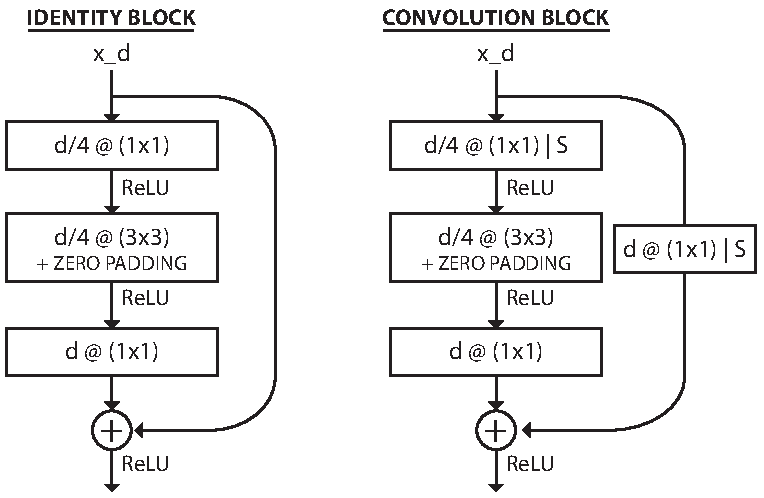
\includegraphics[width=\columnwidth]{resnet-blocks}
    \caption{Building blocks of a ResNet. Identity block is used when input and output dimension are the same, otherwise the convolution block is used. \texttt{x_d} indicates the input \texttt{x} of depth \texttt{d}. \texttt{| S} suffix indicates that a custom stride, different from $1 \times 1$ is applied to that convolution.}
    \label{fig:img_resnet}
\end{figure}

In this paper I implement {\it ResNet-50} and I suggest \cite{resnets-2015} for full details on the implementation.\\
This model is achieved by stacking groups of identity blocks and convolutional blocks to form a 50 layer deep network, the topology is described in \tab{m_resnet_table}.

\begin{table*}[]
\captionsetup{font=scriptsize, justification=centering}
\centering
\resizebox{\textwidth}{!}{%
\begin{tabular}{|c|c|c|c|c|c|c|c|c|c|c|c|}
\hline
\multicolumn{1}{|c|}{\textbf{Input}} & \textbf{Conv} & \textbf{BN} & \textbf{ReLU} & \textbf{MP} & \textbf{S1} & \textbf{S2} & \textbf{S3} & \textbf{S4} & \textbf{AP} & \textbf{Flat} & \textbf{Softmax} \\ \hline
1@(6x128) & 32@(1x4) &  &  &  & 
$\begin{bmatrix} 32@(1 \times 1) \\ 32@(3 \times 3) \\ 128@(1 \times 1) \end{bmatrix} \times 3$ &
$\begin{bmatrix} 64@(1 \times 1) \\ 64@(3 \times 3) \\ 256@(1 \times 1) \end{bmatrix} \times 4$ &
$\begin{bmatrix} 128@(1 \times 1) \\ 128@(3 \times 3) \\ 512@(1 \times 1) \end{bmatrix} \times 6$ &
$\begin{bmatrix} 256@(1 \times 1) \\ 256@(3 \times 3) \\ 1024@(1 \times 1) \end{bmatrix} \times 3$ &
1x2 &  & 7 \\ \hline
\end{tabular}%
}
\caption{\texttt{m_resnet} model representation. \texttt{BN} stands for batch normalization, \texttt{MP} for max pooling, \texttt{S1-S4} represent the 4 stages of the identity-convolutional blocks. \texttt{AP} stands for average pooling, pooling is done only along the temporal dimension.}
\label{m_resnet_table}
\end{table*}

\subsection{Stacked denoising convolutional autoencoders (\texttt{m_ae})}
\label{sec:m_ae}
The main building block of this model is the autoencoder, an architecture composed of an encoder and a decoder. In this setup, the autoencoders are composed only of convolutional layers. The topology of this setup is represented in \fig{fig:img_ae}. Two autoencoders are stacked together, followed by a \mbox{fully-connected} layer for the final classification.\\

\begin{figure*}[ht]
	\captionsetup{font=scriptsize, justification=centering}
    \centering
	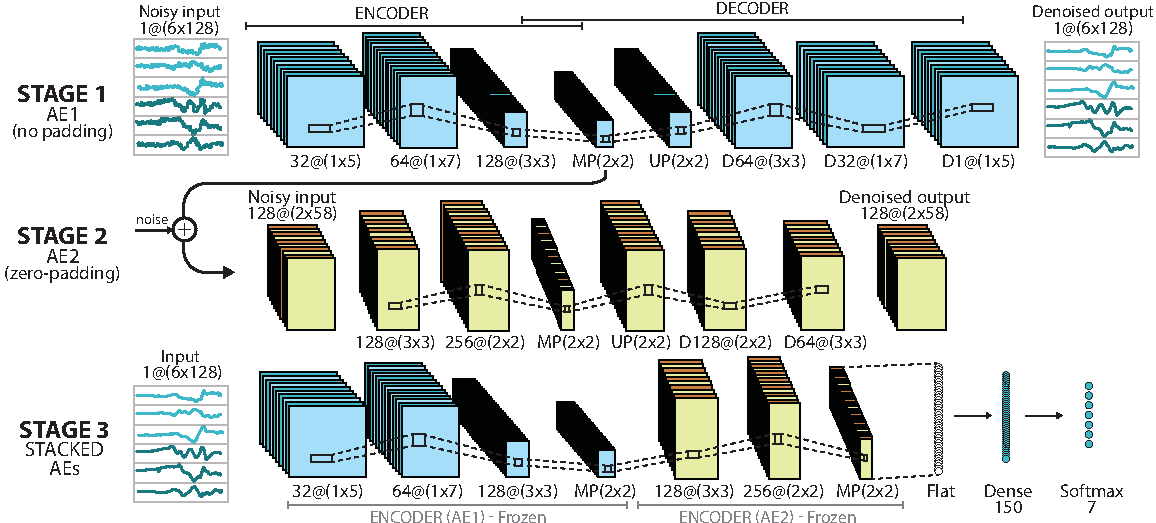
\includegraphics[width=\textwidth]{ae}
    \caption{Processing pipeline of a stacked denoising autoencoder. \texttt{MP} stands for max pooling, \texttt{UP} stands for up scaling, the opposite of a max pooling operation. Operations with \texttt{D} prefix stand for de-convolution operations, which revert the effect of a convolution. Zero-padding indicates that padding was used in order to keep the same feature map size during the various convolution operations.}
    \label{fig:img_ae}
\end{figure*}

Training this kind of models follow a \mbox{two-step} procedure: (i) a corrupted input is used for the initial \mbox{denoising-training} of each individual layer, so that it may learn useful feature extractors. Once the mapping has been learnt, the output of the encoder part (with noisy data given as input) is used as input of the following autoencoder. Noise is always applied to the input of all the autoencoders during training. I tested with two different types of noise, as suggested by \cite{Pascal-2010}:

\begin{itemize}
\item Additive isotropic gaussian noise
\item Masking noise, where a fraction of the elements of the input (chosen at random for each example) is forced to 0. This drastically corrupt a fraction of the elements while leaving the others untouched
\end{itemize}

I also experimented with two different variations of the first autoencoder: this first one being represented in \fig{fig:img_ae} (\texttt{ae-long}) and another one that featured a shallower first autoencoder (\texttt{ae-short}), without an intermediate convolutional layer.

The network parameters of the autoencoders are optimized by minimizing the mean squared error loss function:
$$MSE = \frac{1}{n} \sum_{i=1}^{n}(y_i - \hat{y_i})^2$$

Once a stack of encoders has thus been trained, its output representation can be used as input to a \mbox{stand-alone} supervised learning algorithm. (ii) An output layer is added on top of the stack and the parameters of the whole system are \mbox{fine-tuned} to minimize the error in predicting the supervised target by performing gradient descent. It's important to note that during the \mbox{fine-tuning} phase the uncorrupted inputs are used and the layers of the stacked autoencoders are frozen i.e. no training is performed on these layers, only the weights on the output layers are updated.